\documentclass[11pt]{article}

\usepackage[margin=1in]{geometry}
\usepackage{graphicx}
\usepackage{booktabs}
\usepackage{amsmath}
\usepackage{hyperref}
\usepackage{caption}

\graphicspath{{figures/}}

\title{CSE 620: Combinatorial Optimization\\
\large Simulated Annealing Micro-Project Report}
\author{Your Name \\ University of Louisville}
\date{\today}

\begin{document}
\maketitle

\section*{1. Simulated Annealing: Why It Beats Classical Local Search}
\addcontentsline{toc}{section}{1. Simulated Annealing}

Simulated annealing (SA) is a stochastic local-search heuristic that explores a
solution space by repeatedly moving to a neighboring state, accepting every
improving move and accepting a worsening move of size $\Delta E$ with
probability $\exp(-\Delta E / T)$, where $T$ is a ``temperature'' that is
gradually reduced according to a cooling schedule. Early in the search, a high
$T$ makes uphill moves almost always acceptable, so the algorithm behaves like a
random walk and explores many basins of attraction; as $T \to 0$ the acceptance
probability of worse moves vanishes and the search settles into the best basin
it has found, i.e.\ it exploits. This is precisely what classical methods
cannot do: hill climbing and gradient descent are greedy and only accept
improving moves, so they are guaranteed to terminate at whatever local optimum
(or stationary point) happens to be closest to the starting state, and they
require a good initial guess and (for gradient descent) a differentiable
objective. Because SA retains a non-zero probability of escaping a local
optimum while the temperature is still high, and because a slowly decaying
schedule lets it sample the landscape like a Markov chain before freezing, it
can reach states that greedy search can never leave --- giving it a much better
(approaching global, in the limit of logarithmic cooling) approximation of the
global optimum, at the price of longer run times and a few extra parameters
($T_0$, $\alpha$, schedule type) that must be tuned.

\section*{2. Experiment 1 --- Exponential Cooling Schedule}

Exponential decay cools the temperature as
\begin{equation}
    T_k = T_0 \, \alpha^k ,
\end{equation}
where $T_0$ is the starting temperature and $\alpha \in (0,1)$ is the decay
rate. The following table reports the results of running Section 1 of the
provided notebook (15-city TSP instance generated with
\texttt{random\_state=254}, SA seeded with \texttt{random\_state=192}, averaged
over 10 runs per configuration, stopping at $T < 10^{-5}$).

\begin{table}[h]
\centering
\caption{Exponential decay: average time and best cost over 10 runs.}
\label{tab:exp}
\begin{tabular}{cccr}
\toprule
Starting Temperature & Alpha & Average Time (ms) & Best Cost \\
\midrule
4000 & 0.95 & 330.38  & 2504.8 \\
2000 & 0.95 & 309.17  & 3434.4 \\
4000 & 0.60 & 33.14   & 3963.2 \\
2000 & 0.60 & 37.58   & 3963.2 \\
4000 & 0.30 & 15.26   & 4393.6 \\
2000 & 0.30 & 14.13   & 4178.4 \\
\bottomrule
\end{tabular}
\end{table}

\textbf{Observations.} Both parameters control the same underlying quantity ---
the number of iterations performed, since exponential cooling reaches the
$10^{-5}$ stop temperature after only $k_{\max} = \ln(10^{-5}/T_0)/\ln\alpha$
steps (about 400 steps for $\alpha = 0.95$, but only $\sim$40 and $\sim$17
steps for $\alpha = 0.60$ and $0.30$). There is a clear positive correlation
between $\alpha$ (and, more weakly, $T_0$) and solution quality, as
visualized in Figure~\ref{fig:cooling}: the slowest
schedule, $T_0 = 4000,\ \alpha = 0.95$, found the best tour (2504.8) while the
fastest schedules terminated after a dozen steps and returned tours of
4200--4400, i.e.\ roughly 75\% worse, in under 16 ms. Runtime grows with
$\alpha$ far more than with $T_0$: at $\alpha = 0.30$ the two starting
temperatures are almost indistinguishable, because the temperature has crashed
to zero in a handful of iterations no matter where it started, so $T_0$ only
sets the acceptance probability of the first few moves. At $\alpha = 0.95$,
raising $T_0$ from 2000 to 4000 improves the cost from 3434.4 to 2504.8 for
essentially the same runtime, because a hotter start keeps uphill moves
acceptable longer and lets the search cross higher energy barriers before it
freezes.

\section*{3. Experiment 2 --- Linear Cooling Schedule}

Linear decay cools the temperature as
\begin{equation}
    T_k = \frac{T_0}{1 + \alpha k},
\end{equation}
so the temperature now decreases hyperbolically instead of geometrically. The
experiment from Section 2 was repeated with the same instance, seeds and
averaging protocol, stopping at $T < 1$ as specified in the notebook.

\begin{table}[h]
\centering
\caption{Linear decay: average time and best cost over 10 runs.}
\label{tab:lin}
\begin{tabular}{cccr}
\toprule
Starting Temperature & Alpha & Average Time (ms) & Best Cost \\
\midrule
4000 & 0.95 & 3631.96  & 2477.6 \\
2000 & 0.95 & 1772.89  & 3753.6 \\
4000 & 0.60 & 5444.18  & 2477.6 \\
2000 & 0.60 & 2798.65  & 2894.4 \\
4000 & 0.30 & 10949.77 & 2559.2 \\
2000 & 0.30 & 5213.73  & 2477.6 \\
\bottomrule
\end{tabular}
\end{table}

\begin{figure}[h]
\centering
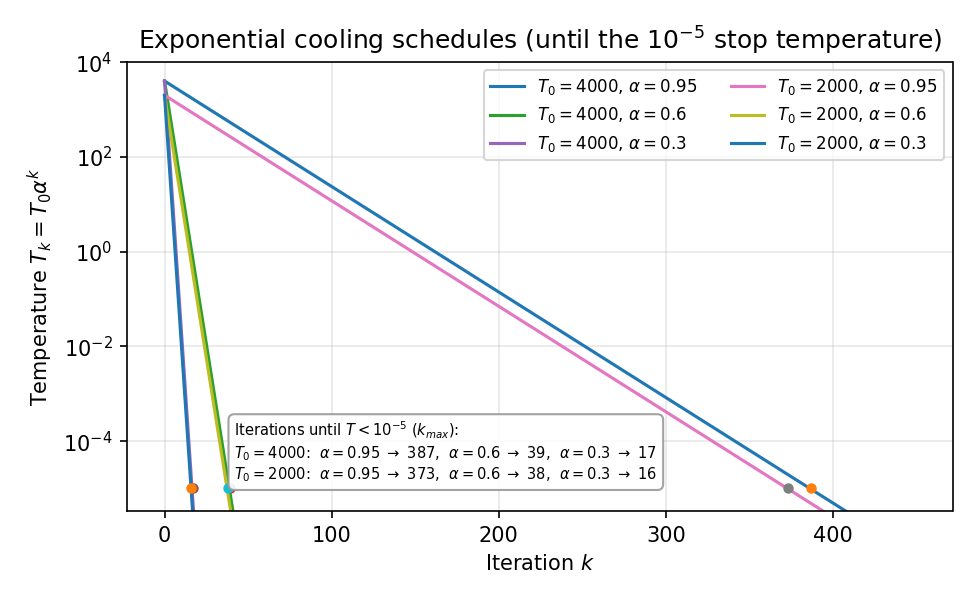
\includegraphics[width=0.72\textwidth]{cooling_curves.png}
\caption{The six exponential schedules tested: a larger $\alpha$ (or larger
$T_0$) keeps the temperature high for many more iterations --- each dot marks
where a schedule crosses the $10^{-5}$ stopping threshold, i.e.\ the number of
iterations that configuration performs.}
\label{fig:cooling}
\end{figure}

\textbf{Observations.} Linear cooling is dramatically slower than exponential
cooling: reaching the stop temperature now takes $k_{\max} \approx (T_0-1)/\alpha$
iterations --- roughly 4200 steps for $T_0 = 4000,\ \alpha = 0.95$ and over
13\,000 steps for $T_0 = 4000,\ \alpha = 0.30$ --- so run times jump from tens
of milliseconds to 1.8--11 seconds, while the best cost drops from 2504.8
(exp) to 2477.6. Note that the role of $\alpha$ is inverted relative to
exponential decay: because $\alpha$ sits in the denominator, a \emph{larger}
$\alpha$ cools \emph{faster}, so run time now \emph{decreases} with $\alpha$
and \emph{increases} with $T_0$. Quality still correlates with the number of
iterations performed --- every configuration that ran at least $\sim$4200 steps
reached the best cost of 2477.6, while the shortest run (2000/0.95, $\sim$2100
steps) finished at 3753.6 --- but the relationship saturates: 13\,000 steps
costs 2.5$\times$ more time than 4200 steps for no gain (2559.2 vs.\ 2477.6,
within stochastic noise). In other words, with linear decay the budget is
controlled by $T_0/\alpha$, and once enough iterations have been spent for the
temperature to become low, extra searching is wasted computation.

\section*{4. Experiment 3 --- Simulated Annealing vs.\ Hill Climbing}

The best parameter combination from the two tables above is the linear schedule
with $T_0 = 4000$ and $\alpha = 0.95$ (best cost 2477.6, and the cheapest of
the three configurations that tie at that cost). It was used to solve randomly
generated instances of 5, 20 and 30 cities (same
\texttt{random\_state=254} generator) and compared against the greedy hill
climber from the notebook on the identical instance.

\begin{table}[h]
\centering
\caption{Simulated annealing (best parameters) vs.\ hill climbing.}
\label{tab:sa-hc}
\begin{tabular}{cccccc}
\toprule
 & \multicolumn{2}{c}{Simulated Annealing} & \multicolumn{2}{c}{Hill Climbing} \\
\cmidrule(lr){2-3}\cmidrule(lr){4-5}
\# Cities & Time (ms) & Cost & Time (ms) & Cost \\
\midrule
5  & 550.64    & 1478.4 & 0.36  & 1478.4 \\
20 & 6511.61   & 4892.0 & 20.29 & 5030.4 \\
30 & 14606.29  & 6967.2 & 44.50 & 7619.2 \\
\bottomrule
\end{tabular}
\end{table}

\begin{figure}[h]
\centering
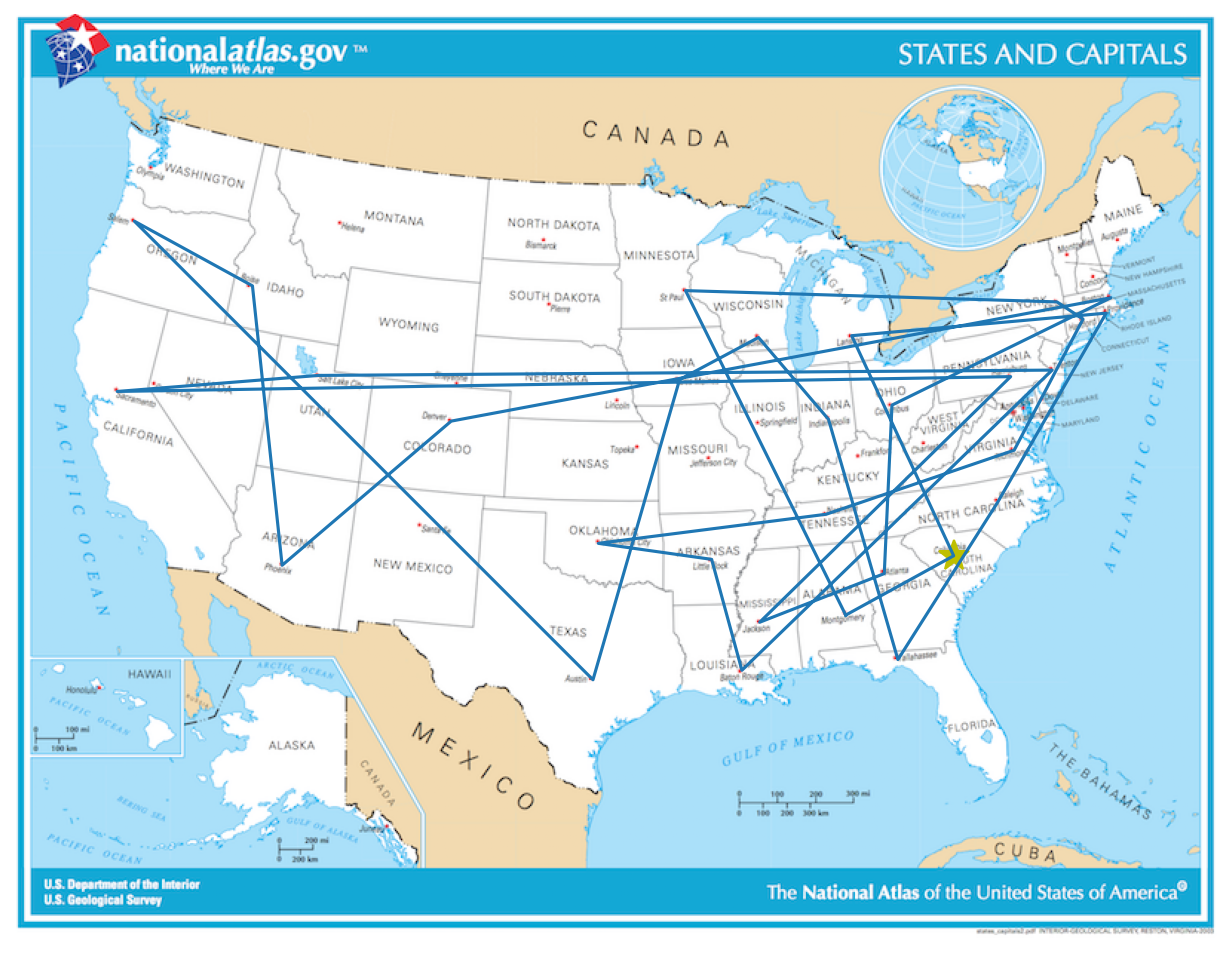
\includegraphics[width=0.85\textwidth]{sa_path_30.png}
\caption{Best 30-city tour found by simulated annealing (linear schedule,
$T_0 = 4000$, $\alpha = 0.95$) on the US capitals map.}
\label{fig:path30}
\end{figure}

\textbf{Observations.} For both algorithms the run time grows with the number
of cities --- SA because it performs a fixed (temperature-driven) number of
iterations whose per-step cost is $O(n^2)$, hill climbing because each greedy
sweep evaluates an $n$-element neighborhood --- but they grow on completely
different scales: SA needs 0.55 s, 6.5 s and 14.6 s for 5, 20 and 30 cities,
while hill climbing needs 0.4 ms, 20 ms and 45 ms, i.e.\ it is 3--4 orders of
magnitude faster throughout. In terms of quality, both algorithms find the
same tour for 5 cities (1478.4), because a 5-city neighborhood graph is tiny
and the greedy search reaches the global optimum anyway; as the instance grows,
hill climbing freezes in the first local optimum it meets and its cost
deteriorates relative to SA: it is 2.8\% worse at 20 cities (5030.4 vs.\
4892.0) and 9.4\% worse at 30 cities (7619.2 vs.\ 6967.2), and the gap keeps
widening with $n$. For the largest problem sizes, therefore, the best approach
is simulated annealing with a slowly cooling schedule, since solution quality
--- not run time --- is what dominates the total routing cost, and exact
methods would be out of reach anyway (TSP is NP-hard). For the smallest
instance, SA is not worth it: hill climbing returns the same optimal tour
about 1500$\times$ faster, so the extra stochastic exploration (and its
parameter tuning) buys nothing.

\section*{5. Concluding Remarks}

Parameter and schedule selection make a very significant difference in the
effectiveness of simulated annealing. Holding everything else fixed, merely
changing $\alpha$ from 0.95 to 0.30 under exponential cooling degraded the
tour from 2504.8 to 4393.6 --- a 75\% worse solution --- while changing the
cooling schedule from exponential to linear improved the best cost from 2504.8
to 2477.6 but at a 100-fold increase in run time (0.33 s vs.\ 3.6 s), showing
that the schedule controls how the search budget is spent: fast cooling is
cheap but premature and greedy-like, slow cooling explores but can waste
iterations once the temperature is already low (the 13\,000-step linear run
gained nothing over the 4\,200-step run). Starting temperature matters mainly
through the number of iterations it sustains and the acceptance rate it
produces early on; it is only consequential when the decay rate is slow enough
for the run to last (at $\alpha = 0.30$ the two $T_0$ values were almost
indistinguishable). The comparison with hill climbing also showed that the
extra effort pays off exactly where it should: SA and hill climbing tie on the
tiny instance, but SA's ability to accept uphill moves yields progressively
better tours as the problem grows. In short, SA's superiority is not free ---
it is earned through a sensible choice of $T_0$, $\alpha$ and cooling
schedule, and that choice, not the algorithm itself, is what determines
whether the result is a near-optimal tour or a mediocre one.

\section*{Appendix: Reproducibility}

All experiments were run with the code of \texttt{CSE620\_SA\_Project\_Notebook.ipynb}
unchanged (problem definition, \texttt{Schedule} class,
\texttt{simulated\_annealing()} and \texttt{hill\_climbing()} implementations),
driven by the helper script \texttt{experiments.py} in a dedicated Python
environment (\texttt{.venv}, listed in \texttt{.gitignore}). Cities are drawn
with \texttt{np.random.default\_rng(254)}, every SA run uses
\texttt{random\_state=192}, and every reported time is the mean of 10 runs.
The provided sanity-check entries were reproduced exactly in cost
($3963.2$ for exponential 2000/0.60 and $2894.4$ for linear 2000/0.60); wall
clock times differ from the reference machine by roughly 30\% but are
internally consistent, since all configurations were timed on the same
machine.

\end{document}
